\documentclass[authoryear, review, 11pt]{elsarticle}

\setlength{\textwidth}{6.5in}
%\setlength{\textheight}{9in}
\setlength{\topmargin}{0in}
\setlength{\oddsidemargin}{0in}
\setlength{\evensidemargin}{0in}

\usepackage{amsmath}
\usepackage{amsthm}
\usepackage{amssymb}
\usepackage{mathabx}
\usepackage{bm}
\usepackage{multirow}

%\geometry{landscape}                % Activate for for rotated page geometry
\usepackage[parfill]{parskip}    % Activate to begin paragraphs with an empty line rather than an indent
\usepackage{graphicx}
\usepackage{epstopdf}
\usepackage{natbib}
\usepackage{verbatim}
\usepackage{longtable}
\usepackage{rotating}
\usepackage[nolists,nomarkers]{endfloat}
\DeclareDelayedFloatFlavour{sidewaystable}{table}

\usepackage{relsize}
%\usepackage{caption}
\usepackage{subcaption}
\usepackage{fullpage}
\usepackage{booktabs}


\usepackage{setspace}
\setstretch{2}

\DeclareGraphicsRule{.tif}{png}{.png}{`convert #1 `dirname #1`/`basename #1 .tif`.png}
\DeclareMathOperator*{\argmin}{\arg\!\min}
\DeclareMathOperator*{\argmax}{\arg\!\max}
\DeclareMathOperator*{\bw}{\mbox{bw}}
\DeclareMathOperator*{\df}{\mbox{df}}
\newcommand{\vect}[1]{\bm{#1}}
\newcommand{\E}{\mathop{\mathbb E}}


\title{Local Variable Selection and Parameter Estimation of Spatially Varying Coefficient Regression Models}
\author{Wesley Brooks}
\date{}                                           % Activate to display a given date or no date

\begin{document}
\maketitle

\section{Simulation \label{sec:simulation}}
	\begin{comment}

	\subsection{Simulation Setup}
	A simulation study was conducted to assess the performance of the method described in Sections \ref{section:GWR}--\ref{section:model-selection}. 
	
	Data were simulated on the spatial domain $[0,1]^2$, which was divided into a $30 \times 30$ grid. Each of $p=5$ covariates $X_1, \dots, X_5$ was simulated by a Gaussian random field (GRF) with mean zero and exponential spatial covariance $\text{Cov} \left(X_{ji}, X_{ji'} \right) = \sigma_x^2 \exp{\left( -\tau_x^{-1} \delta_{ii'} \right)}$ where $\sigma_x^2=1$ is the variance, $\tau_x = 0$ is the range parameter, and $\delta_{ii'}$ is the Euclidean distance $\|\bm{s}_i - \bm{s}_{i'}\|_2$. Correlation was induced between the covariates by multiplying the $\bm{X}$ matrix by $\bm{R}$, where $\bm{R}$ is the Cholesky decomposition of the covariance matrix $\bm{\Sigma} = \bm{R}'\bm{R}$. The covariance matrix $\bm{\Sigma}$ is a $5 \times 5$ matrix that has ones on the diagonal and $\rho$ for all off-diagonal entries, where $\rho$ is the between-covariate correlation.
		
	The simulated response was $y_i = \bm{x}'_i \bm{\beta}_i + \varepsilon_i$ for $i=1, \dots, n$ where $n=900$ and for simplicity the $\varepsilon_i$'s were iid Gaussian with mean zero and variance $\sigma_\varepsilon^2$. The simulated data included the response $y$ and five covariates $x_1, \dots, x_5$. The true data-generating model uses only $x_1$, so $x_2, \dots, x_5$ are included to assess performance in variable-selection.
	
	There were twelve simulation settings, each of which was simulated 100 times. For each of the twelve settings, $\beta_1(\bm{s})$, the true coefficient surface for $x_1$, was nonzero in at least part of the spatial domain $[0,1]^2$. There were four other simulated covariates, but their true coefficient surfaces were zero across the area under simulation. The twelve simulation settings are described in Table \ref{table:simulation_settings}. Three parameters were varied to produce the twelve settings: there were three functional forms for the coefficient surface $\beta_1(\bm{s})$, data was simulated both with ($\rho = 0.5$) and without ($\rho = 0$) correlation between the covariates, and simulations were made with low ($\sigma_\varepsilon^2 = 0.25$) and high ($\sigma_\varepsilon^2 = 1$) variance for the random error term.
	
	The three coefficient surfaces used to produce the response variable in the simulations are pictured in Figure \ref{fig:sim-actual}. The first is a ``step" function, which is equal to zero in 40\% of the spatial domain, equal to one in a different 40\% of the spatial domain, and increases linearly in the middle 20\% of the domain. The second is a gradient function, which increases linearly from zero at one end of the domain to one at the other. The final coefficient function is a parabola taking its maximum value of 0.535 at the center of the domain and falling to zero at each corner of the domain. The parabola is computed by finding the squared distance of each sampling location from the domain's center, multiplying by -1 and then adding an offset so that the corner points are equal to zero.
	
	The performance of the penalized GWR methods (AL via {\tt lars} and via {\tt glmnet}, and the AEN  via {\tt enet}) was compared to that of oracular GWR (O-GWR), which is ordinary GWR with ``oracular" variable selection, meaning that exactly the correct set of covariates was used to fit the GWR model at each location in the simulation. Also included in the comparison was the GWR algorithm of \cite{Fotheringham:2002} without variable selection ({\tt gwr}). Finally, there is a category of simulation results using the three penalized GWR methods for local variable selection and then ordinary GWR for coefficient estimation.
	
	\end{comment}
	
% latex table generated in R 2.15.1 by xtable 1.7-0 package
% Fri Jan 18 10:19:47 2013
\begin{table}[h!]
	\begin{center}
	\begin{tabular}{cccc}
		\hline
		Setting & function & $\rho$ & $\sigma^2$ \\ 
		\hline
		1 & step & 0 & 0.25 \\ 
		2 & step & 0 & 1 \\ 
		3 & step & 0.5 & 0.25 \\ 
		4 & step & 0.5 & 1 \\ 
		\hline
		5 & gradient & 0 & 0.25 \\ 
		6 & gradient & 0 & 1 \\ 
		7 & gradient & 0.5 & 0.25 \\ 
		8 & gradient & 0.5 & 1 \\ 
		\hline
		9 & parabola & 0 & 0.25 \\ 
		10 & parabola & 0 & 1 \\ 
		11 & parabola & 0.5 & 0.25 \\ 
		12 & parabola & 0.5 & 1 
	\end{tabular}
	\end{center}
	\caption{Simulation parameters for each setting.\label{table:simulation_settings}}
\end{table}

	\begin{figure}
		\begin{center}
			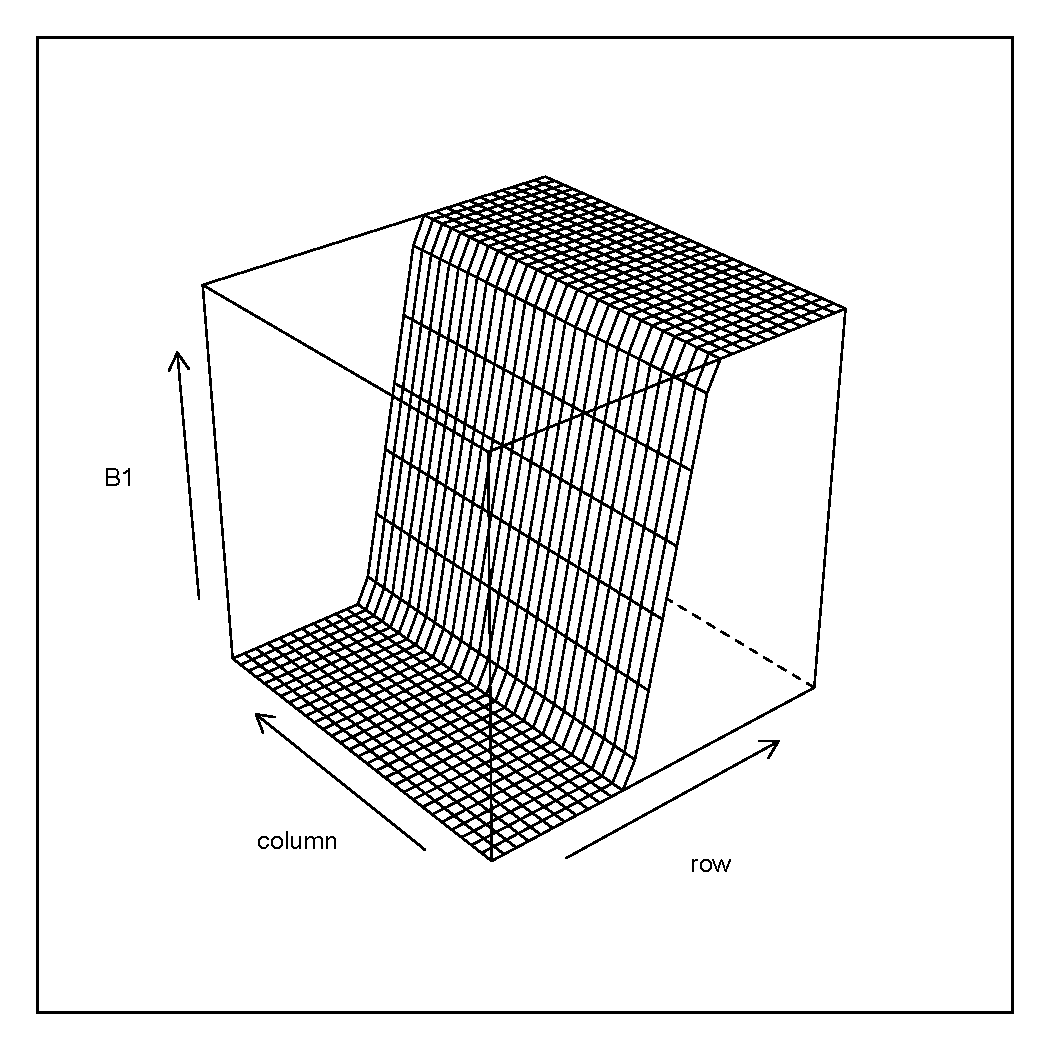
\includegraphics[width=0.32\textwidth]{../../figures/simulation/step.pdf}
			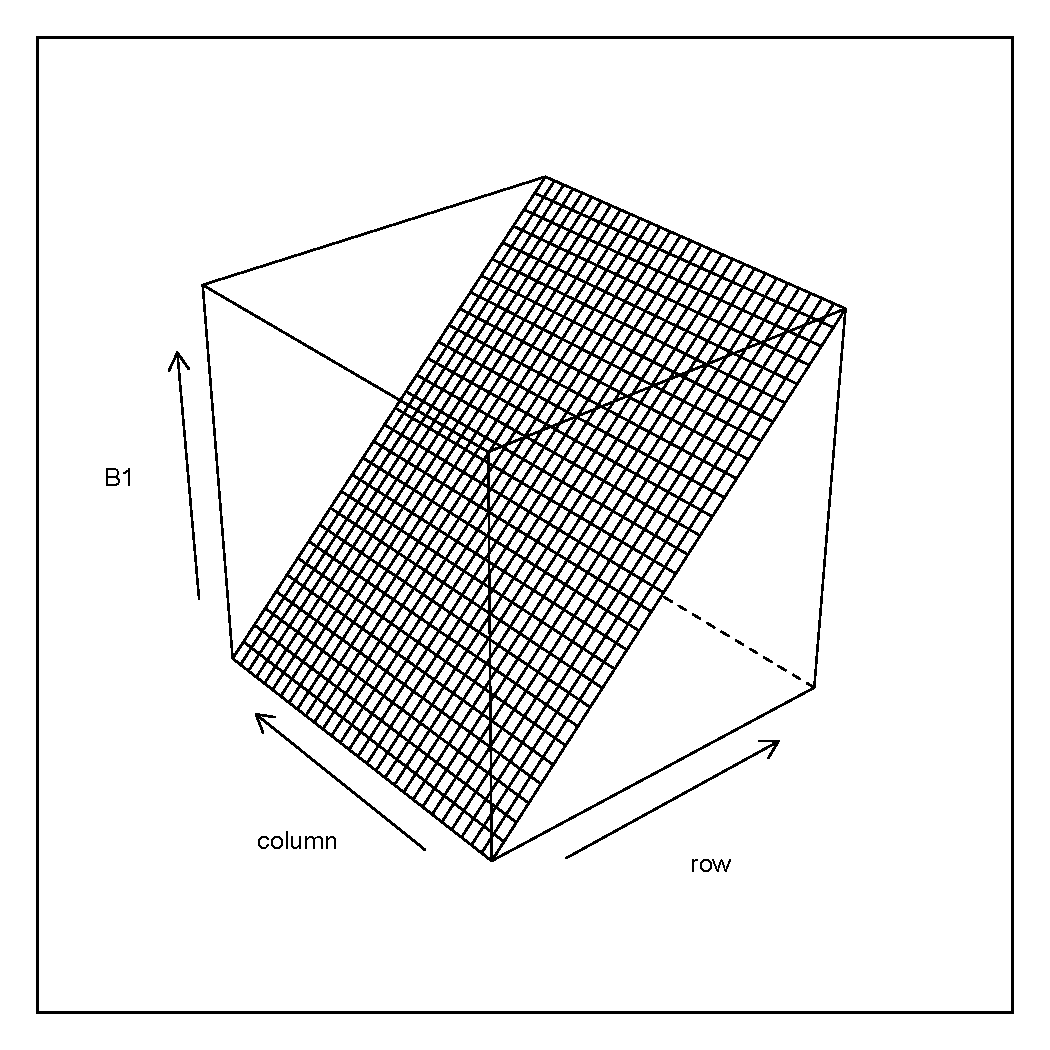
\includegraphics[width=0.32\textwidth]{../../figures/simulation/gradient.pdf}
			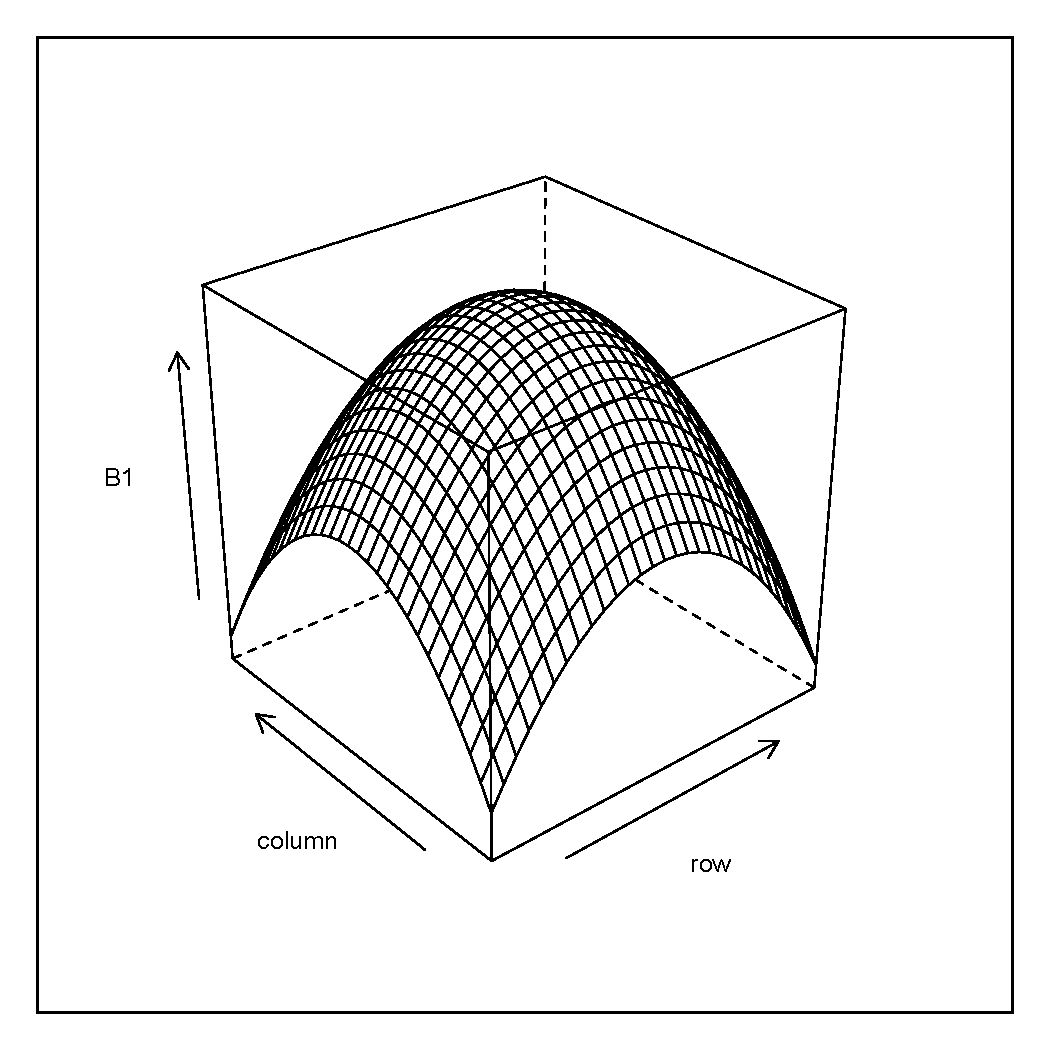
\includegraphics[width=0.32\textwidth]{../../figures/simulation/parabola.pdf}
			\caption{The actual $\beta_1$ coefficient surface used in the simulation.\label{fig:sim-actual}}
		\end{center}
	\end{figure}
	
	\begin{figure}
		\begin{center}
			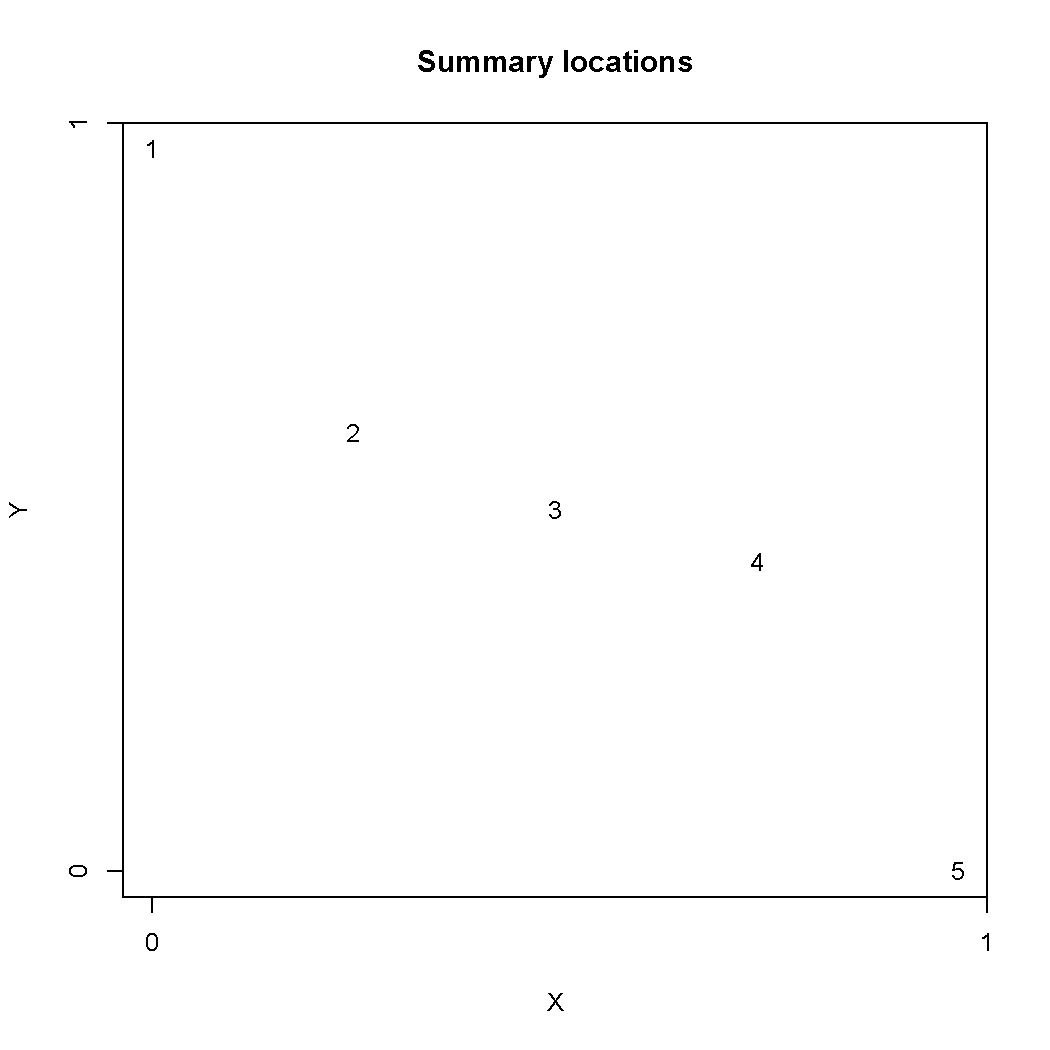
\includegraphics[width=0.5\textwidth]{../../figures/simulation/illustrations/summary-locations.pdf}
			\caption{Locations where the variable selection and coefficient estimation of GWL were summarized.\label{fig:summary-locations}}
		\end{center}
	\end{figure}
	
	
	Results from the simulation were summarized at five locations on the simulated grid (see Figure \ref{fig:summary-locations}). The five key locations were chosen because they represent interesting regions of the $\beta_1$ coefficient surfaces. The results of variable selection and coefficient estimation are presented in the tables below.
	
	%Results of the simulation experiment were summarized to asses the consistency in selection and estimation, as well as the coverage properties of the confidence intervals. The confidence intervals based on the bootstrap (without shrinkage) were used for the GWL because they seemed to uniformly outperform the other options.\\ table:loc1-X1-BiasX
	
		\begin{comment}
	\subsection{Simulation results}
	
	%At locations where $\beta_1$ is nonzero, $X_1$ usually selected for inclusion in all or nearly all of the model runs. An exception is at location four for the step function, where $X_1$ was included in about half of the model runs. This is probably because location four is at the very point where $\beta_1$ transitions from zero to nonzero. Selection performance was relatively poor for the step function at location one, especially for data with $\sigma^2 = 1$. For those simulations, $X_1$ was correctly included in around 85\% of the simulations. The bias, variance, and MSE of $\hat{\beta}_1$ under the same settings were also much larger than the baseline established by the standard \verb!gwr! algorithm. The reason(s) for the poor performance under those particular conditions is currently unknown.\\
	
	\paragraph{Selection} Table \ref{table:selection} lists the results of variable selection. The correct covariate was usually included in the local models, and the unimportant covariates were usually excluded. Arguably the least-accurate selection was at locations one and five for the step function using the {\tt lars} algorithm, where variables that do not appear in the true model were selected for inclusion at rates between 11\% and 22\%. The {\tt enet} and {\tt glmnet} algorithms, using the same data, had false-positive errors at rates between 0\% and 8\%, which are typical of the error rates for all other location/function/algorithm combinations.
	
	Selection performance was more affected by an increase in the noise variance from $\sigma_{\varepsilon}=0.5$ to $\sigma_{\varepsilon}=1$ than by an increase in colinearity from $\rho = 0$ to $\rho = 0.5$. For instance, for the step function at location three, $\beta_1(\bm{s}_3) = 0.5$. Where $\sigma_{\varepsilon}=0.5$, the {\tt glmnet} algorithm selected $\beta_1(\bm{s}_3) $ for inclusion at a rate of 100\% (when $\rho = 0$) and 99\% (when $\rho = 0.5$). But when $\sigma_{\varepsilon}=1$, the same algorithm selected $\beta_1(\bm{s}_3)$ for inclusion at a rate of 75\% (when $\rho = 0$) and 68\% (when $\rho = 0.5$).
	
	The \verb!enet! algorithm outperforms the others in selection but the difference is small - a roughly one percentage point improvement in the rate of true positives and true negatives when $\rho = 0.5$.There is no apparent difference between {\tt glmnet} and {\tt enet} when $\rho = 0$.  
	
	%Otherwise, selection performance was good, with the rate of false positive selections for $X_2$--$X_5$ (and for $X_1$ where its true coefficient was zero) usually below 0.10. Selection (also bias, variance, and MSE of $\hat{\beta}_1(\bm{s})$) tended to suffer worse by the change from low to high error variance than by the change from low to high collinearity amongst the predictors.\\
	
	\paragraph{Coefficient Estimation} The MSE, bias, and variance of $\hat{\beta}_1$ are listed in Tables \ref{table:X1-mse}, \ref{table:X1-bias}, and \ref{table:X1-var}, respectively. The method of oracular selection led to the best MSE in 28 of the 60 cases, which is more than any other single method. In general, the methods that do local variable selection had lower MSE than traditional GWR. As was the case for selection, estimation accuracy (in terms of MSE) suffered more by an increase in $\sigma_{\varepsilon}$ from 0.5 to 1 than from an increase in $\rho$ from 0 to 0.5. Oracular selection was decisively superior to traditional GWR and to local variable selection for estimating the gradient $\beta_1$, turning in the best MSE for all combinations of location and simulation parameters.
	
	In general, oracular selection and traditional GWR were quite similar in terms of $\text{var}\left(\hat{\beta_1}\right)$, with notably greater variance for the local selection methods. However, the local selection methods had less bias than traditional GWR, even exhibiting less bias than oracular selection in many settings. There was no simulation setting for which traditional GWR had the smallest or second-smallest bias.
	
	It seems, therefore, that the local selection methods reduce bias and increase variance of the coefficient estimates, as compared to traditional GWR. Whether traditional GWR or local selection is better in terms of MSE of the coefficient estimates is not clear in all cases, but when the actual coefficient is equal to zero (or nearly so), local selection does seem to reduce the MSE over traditional GWR.
	
	%There was not a clear and consistent difference in performance between the three selection methods. It might be expected that the adaptive elastic net would outperform the adaptive Lasso under greater covariate collinearity, but if such effect is real it is not apparent from this simulation. The unshrunk coefficient-estimation methods tended to exhibit more bias than the selection-plus-shrinkage methods when the true coefficient value was near zero, and vice versa when the true coefficient was not near zero. The unshrunk methods were perhaps more consistent in their performance and for that reason they are probably preferable in practice.\\
	
	%Bias in coefficient estimation was greater and variance less for the standard \verb!gwr! algorithm than for the methods described here. This is probably due to the fact that the methods described here show a preference for smaller bandwidths than those select by \verb!gwr!. Accuracy (as measured by MSE) in fitting the true Y variables was comparable for all the methods. \\	
	
	\paragraph{Fitted Values} The MSE of the $\hat{Y}$, $\text{MSE}\left(\hat{Y}\right)$, is listed in Table \ref{table:Y-mse}. Nominally, $\text{MSE}\left(\hat{Y}\right)$ should be equal to the noise variance, $\sigma_{\varepsilon}^2$, which is 1 for odd-numbered rows and 0.25 for even numbered rows. There is not much difference in $\text{MSE}\left(\hat{Y}\right)$ between the various estimation methods, except that it is larger for the oracular and \verb!gwr! methods where $\beta_1(\bm{s})$ is near or equal to zero.
	
	\end{comment}
	
	\subsection{Tables}
\subsubsection{Selection}
% latex table generated in R 2.15.2 by xtable 1.7-0 package
% Thu Apr 18 16:14:00 2013		
\begin{table}
\thispagestyle{empty}
\begin{center}
\setlength\tabcolsep{4pt}	
\begin{tabular}{ccc|cc|cc|cc|cc|cc}
& \multicolumn{4}{c}{step} & \multicolumn{4}{|c|}{gradient} & \multicolumn{4}{c}{parabola} \\
& \multicolumn{2}{c}{\texttt{enet}} & \multicolumn{2}{c|}{\texttt{glmnet}} & \multicolumn{2}{c}{\texttt{enet}} & \multicolumn{2}{c|}{\texttt{glmnet}}  & \multicolumn{2}{c}{\texttt{enet}} & \multicolumn{2}{c}{\texttt{glmnet}} \\
location & $\beta_1$ & $\beta_2$ - $\beta_5$ & $\beta_1$ & $\beta_2$ - $\beta_5$ & $\beta_1$ & $\beta_2$ - $\beta_5$ & $\beta_1$ & $\beta_2$ - $\beta_5$ & $\beta_1$ & $\beta_2$ - $\beta_5$ & $\beta_1$ & $\beta_2$ - $\beta_5$ \\ 
   \hline
   \multirow{2}{*}{1} & 0.80 & 0.02 & 0.80 & 0.02 & 0.77 & 0.05 & 0.74 & 0.04 & 0.00 & 0.00 & 0.00 & 0.00 \\ 
   & 0.80 & 0.04 & 0.80 & 0.04 & 0.69 & 0.07 & 0.69 & 0.07 & 0.03 & 0.01 & 0.03 & 0.01 \\ 
   \cline{2-13}
   \multirow{2}{*}{2} & 0.97 & 0.00 & 0.98 & 0.00 & 0.80 & 0.01 & 0.80 & 0.00 & 0.51 & 0.01 & 0.49 & 0.01 \\ 
   & 0.96 & 0.01 & 0.96 & 0.01 & 0.63 & 0.04 & 0.64 & 0.03 & 0.46 & 0.01 & 0.46 & 0.01 \\ 
   \cline{2-13}
   \multirow{2}{*}{3} & 0.31 & 0.00 & 0.32 & 0.00 & 0.43 & 0.01 & 0.50 & 0.02 & 0.69 & 0.01 & 0.69 & 0.00 \\ 
   & 0.36 & 0.02 & 0.36 & 0.02 & 0.35 & 0.04 & 0.36 & 0.04 & 0.53 & 0.03 & 0.54 & 0.03 \\ 
   \cline{2-13}
   \multirow{2}{*}{4} & 0.00 & 0.00 & 0.00 & 0.00 & 0.24 & 0.01 & 0.26 & 0.01 & 0.56 & 0.00 & 0.59 & 0.00 \\ 
   & 0.07 & 0.01 & 0.07 & 0.01 & 0.23 & 0.01 & 0.35 & 0.01 & 0.51 & 0.03 & 0.51 & 0.03 \\ 
   \cline{2-13}
   \multirow{2}{*}{5} & 0.01 & 0.00 & 0.01 & 0.00 & 0.00 & 0.00 & 0.00 & 0.00 & 0.01 & 0.01 & 0.01 & 0.01 \\ 
   & 0.03 & 0.01 & 0.03 & 0.01 & 0.02 & 0.03 & 0.04 & 0.03 & 0.03 & 0.03 & 0.02 & 0.03 \\ 
  \end{tabular}
\caption{Selection frequency for the simulation experiment\label{table:selection}}
\end{center}
\end{table}
		


		\subsubsection{Estimation}
		
% latex table generated in R 2.15.2 by xtable 1.7-1 package
% Fri Aug 30 12:27:48 2013
\begin{table}
\thispagestyle{empty}
\begin{center}
\begin{tabular}{cccccccc}
 function & location & enet & glmnet & u.enet & u.glmnet & oracular & gwr \\ 
  \hline
  \multirow{10}{*}{step} & \multirow{2}{*}{1} & 0.241 & \emph{0.239} & 0.520 & 0.520 & 0.514 & \textbf{0.020} \\ 
   &  & 0.289 & \emph{0.287} & 0.781 & 0.780 & 0.899 & \textbf{0.047} \\ 
   \cline{3-8}
   & \multirow{2}{*}{2} & 0.062 & 0.054 & 0.048 & 0.040 & \emph{0.030} & \textbf{0.027} \\ 
   &  & 0.080 & 0.078 & 0.064 & 0.064 & \emph{0.049} & \textbf{0.031} \\ 
   \cline{3-8}
   & \multirow{2}{*}{3} & 0.122 & 0.121 & 0.125 & 0.124 & \emph{0.026} & \textbf{0.008} \\ 
   &  & 0.126 & 0.126 & 0.135 & 0.135 & \emph{0.063} & \textbf{0.017} \\ 
   \cline{3-8}
   & \multirow{2}{*}{4} & \textbf{0.005} & \textbf{0.005} & \textbf{0.005} & \textbf{0.005} & 0.037 & 0.026 \\ 
   &  & \textbf{0.015} & \emph{0.015} & 0.018 & 0.018 & 0.075 & 0.035 \\ 
   \cline{3-8}
   & \multirow{2}{*}{5} & \emph{0.002} & 0.002 & 0.007 & 0.007 & \textbf{0.000} & 0.026 \\ 
   &  & \emph{0.008} & 0.008 & 0.033 & 0.033 & \textbf{0.000} & 0.056 \\ 
   \hline
  \multirow{10}{*}{gradient} & \multirow{2}{*}{1} & 0.317 & 0.321 & 0.599 & 0.573 & \emph{0.291} & \textbf{0.051} \\ 
   &  & 0.376 & \emph{0.360} & 0.550 & 0.558 & 0.615 & \textbf{0.072} \\ 
   \cline{3-8}
   & \multirow{2}{*}{2} & 0.319 & 0.277 & 0.251 & 0.250 & \textbf{0.115} & \emph{0.116} \\ 
   &  & 0.438 & 0.396 & 0.383 & 0.365 & \textbf{0.153} & \emph{0.154} \\ 
   \cline{3-8}
   & \multirow{2}{*}{3} & 0.106 & 0.096 & 0.112 & 0.104 & \emph{0.027} & \textbf{0.016} \\ 
   &  & 0.125 & 0.129 & 0.138 & 0.138 & \emph{0.054} & \textbf{0.027} \\ 
   \cline{3-8}
   & \multirow{2}{*}{4} & \textbf{0.038} & \emph{0.056} & 0.058 & 0.074 & 0.138 & 0.132 \\ 
   &  & \textbf{0.053} & \emph{0.079} & 0.083 & 0.122 & 0.164 & 0.150 \\ 
   \cline{3-8}
   & \multirow{2}{*}{5} & \textbf{0.000} & \textbf{0.000} & \textbf{0.000} & \textbf{0.000} & \textbf{0.000} & 0.041 \\ 
   &  & \emph{0.006} & 0.022 & 0.024 & 0.113 & \textbf{0.000} & 0.061 \\ 
   \hline
  \multirow{10}{*}{parabola} & \multirow{2}{*}{1} & \emph{1.000} & \emph{1.000} & \emph{1.000} & \emph{1.000} & 1.373 & \textbf{0.751} \\ 
   &  & \emph{1.018} & 1.018 & 1.063 & 1.063 & 1.670 & \textbf{0.726} \\ 
   \cline{3-8}
   & \multirow{2}{*}{2} & 0.179 & 0.184 & 0.173 & 0.180 & \emph{0.035} & \textbf{0.026} \\ 
   &  & 0.197 & 0.197 & 0.199 & 0.199 & \emph{0.056} & \textbf{0.024} \\ 
   \cline{3-8}
   & \multirow{2}{*}{3} & 0.077 & 0.077 & 0.083 & 0.082 & \emph{0.018} & \textbf{0.007} \\ 
   &  & 0.127 & 0.125 & 0.144 & 0.142 & \emph{0.047} & \textbf{0.012} \\ 
   \cline{3-8}
   & \multirow{2}{*}{4} & 0.084 & 0.078 & 0.095 & 0.089 & \emph{0.030} & \textbf{0.009} \\ 
   &  & 0.111 & 0.112 & 0.129 & 0.129 & \emph{0.062} & \textbf{0.017} \\ 
   \cline{3-8}
   & \multirow{2}{*}{5} & 0.006 & 0.006 & \textbf{0.005} & \textbf{0.005} & 0.261 & 0.046 \\ 
   &  & \emph{0.011} & \textbf{0.008} & 0.029 & 0.027 & 0.538 & 0.079 \\ 
  \end{tabular}
\caption{Mean squared error of $\hat{\beta_1}$ (\textbf{minimum}, \emph{next best}).\label{table:X1-mse}}
\end{center}
\end{table}
		

% latex table generated in R 2.15.2 by xtable 1.7-1 package
% Fri Aug 30 12:27:48 2013
\begin{table}
\thispagestyle{empty}
\begin{center}
\begin{tabular}{cccccccc}
 function & location & enet & glmnet & u.enet & u.glmnet & oracular & gwr \\ 
  \hline
  \multirow{10}{*}{step} & \multirow{2}{*}{1} & -0.221 & -0.214 & \emph{-0.052} & -0.053 & 0.062 & \textbf{0.014} \\ 
   &  & -0.250 & -0.242 & \emph{-0.017} & \textbf{-0.016} & 0.139 & 0.024 \\ 
   \cline{3-8}
   & \multirow{2}{*}{2} & -0.129 & -0.121 & -0.063 & \emph{-0.057} & \textbf{-0.033} & -0.129 \\ 
   &  & -0.142 & -0.137 & \emph{-0.042} & -0.042 & \textbf{0.001} & -0.135 \\ 
   \cline{3-8}
   & \multirow{2}{*}{3} & -0.263 & -0.257 & -0.251 & -0.247 & \textbf{-0.011} & \emph{0.016} \\ 
   &  & -0.231 & -0.231 & -0.193 & -0.192 & \textbf{0.002} & \emph{0.019} \\ 
   \cline{3-8}
   & \multirow{2}{*}{4} & \textbf{-0.069} & \textbf{-0.069} & \textbf{-0.069} & \textbf{-0.069} & 0.083 & 0.132 \\ 
   &  & -0.038 & -0.037 & \emph{-0.034} & -0.034 & \textbf{0.024} & 0.130 \\ 
   \cline{3-8}
   & \multirow{2}{*}{5} & \emph{0.005} & 0.005 & 0.009 & 0.009 & \textbf{0.000} & -0.013 \\ 
   &  & \emph{0.002} & 0.002 & 0.005 & 0.005 & \textbf{0.000} & -0.018 \\ 
   \hline
  \multirow{10}{*}{gradient} & \multirow{2}{*}{1} & -0.334 & -0.286 & -0.148 & -0.169 & \textbf{0.011} & \emph{-0.054} \\ 
   &  & -0.414 & -0.351 & -0.135 & -0.135 & \textbf{0.050} & \emph{-0.054} \\ 
   \cline{3-8}
   & \multirow{2}{*}{2} & -0.514 & -0.464 & -0.420 & -0.418 & \textbf{-0.317} & \emph{-0.320} \\ 
   &  & -0.597 & -0.545 & -0.514 & -0.494 & \textbf{-0.342} & \emph{-0.364} \\ 
   \cline{3-8}
   & \multirow{2}{*}{3} & -0.221 & -0.166 & -0.178 & -0.131 & \textbf{0.061} & \emph{0.066} \\ 
   &  & -0.238 & -0.212 & -0.197 & -0.184 & \textbf{0.033} & \emph{0.051} \\ 
   \cline{3-8}
   & \multirow{2}{*}{4} & \textbf{0.037} & \emph{0.058} & 0.060 & 0.077 & 0.335 & 0.348 \\ 
   &  & \textbf{0.049} & 0.108 & \emph{0.079} & 0.151 & 0.329 & 0.353 \\ 
   \cline{3-8}
   & \multirow{2}{*}{5} & \textbf{0.000} & \textbf{0.000} & \textbf{0.000} & \textbf{0.000} & \textbf{0.000} & 0.018 \\ 
   &  & \emph{0.009} & 0.019 & 0.015 & 0.042 & \textbf{0.000} & 0.066 \\ 
   \hline
  \multirow{10}{*}{parabola} & \multirow{2}{*}{1} & \emph{-1.000} & \emph{-1.000} & \emph{-1.000} & \emph{-1.000} & -1.066 & \textbf{-0.851} \\ 
   &  & -0.998 & -0.998 & -1.004 & -1.004 & \emph{-0.974} & \textbf{-0.823} \\ 
   \cline{3-8}
   & \multirow{2}{*}{2} & -0.331 & -0.335 & -0.298 & -0.308 & \textbf{-0.105} & \emph{-0.132} \\ 
   &  & -0.357 & -0.354 & -0.320 & -0.320 & \emph{-0.136} & \textbf{-0.128} \\ 
   \cline{3-8}
   & \multirow{2}{*}{3} & -0.129 & -0.128 & -0.087 & -0.086 & \emph{0.041} & \textbf{0.031} \\ 
   &  & -0.187 & -0.181 & -0.122 & -0.115 & \emph{0.042} & \textbf{0.027} \\ 
   \cline{3-8}
   & \multirow{2}{*}{4} & -0.137 & -0.124 & -0.092 & \emph{-0.079} & 0.085 & \textbf{0.052} \\ 
   &  & -0.135 & -0.136 & -0.081 & -0.082 & \emph{0.067} & \textbf{0.048} \\ 
   \cline{3-8}
   & \multirow{2}{*}{5} & 0.008 & 0.008 & \textbf{0.007} & \textbf{0.007} & 0.101 & 0.159 \\ 
   &  & \emph{0.018} & \textbf{0.013} & 0.024 & 0.019 & 0.102 & 0.171 \\ 
  \end{tabular}
\caption{Bias of $\hat{\beta_1}$ (\textbf{minimum}, \emph{next best}).\label{table:X1-bias}}
\end{center}
\end{table}		



% latex table generated in R 2.15.2 by xtable 1.7-1 package
% Fri Aug 30 12:27:48 2013
\begin{table}
\thispagestyle{empty}
\begin{center}
\begin{tabular}{cccccccc}
 function & location & enet & glmnet & u.enet & u.glmnet & oracular & gwr \\ 
  \hline
  \multirow{10}{*}{step} & \multirow{2}{*}{1} & \emph{0.194} & 0.196 & 0.523 & 0.523 & 0.515 & \textbf{0.020} \\ 
   &  & \emph{0.229} & 0.231 & 0.788 & 0.788 & 0.889 & \textbf{0.046} \\ 
   \cline{3-8}
   & \multirow{2}{*}{2} & 0.045 & 0.039 & 0.044 & 0.037 & \emph{0.029} & \textbf{0.011} \\ 
   &  & 0.060 & 0.060 & 0.063 & 0.063 & \emph{0.049} & \textbf{0.013} \\ 
   \cline{3-8}
   & \multirow{2}{*}{2} & 0.054 & 0.055 & 0.063 & 0.063 & \emph{0.026} & \textbf{0.008} \\ 
   &  & 0.073 & 0.074 & 0.099 & 0.099 & \emph{0.064} & \textbf{0.017} \\ 
   \cline{3-8}
   & \multirow{2}{*}{2} & \textbf{0.000} & \textbf{0.000} & \textbf{0.000} & \textbf{0.000} & 0.030 & 0.009 \\ 
   &  & \textbf{0.013} & \emph{0.013} & 0.017 & 0.017 & 0.075 & 0.019 \\ 
   \cline{3-8}
   & \multirow{2}{*}{2} & \emph{0.002} & 0.002 & 0.007 & 0.007 & \textbf{0.000} & 0.027 \\ 
   &  & \emph{0.008} & 0.008 & 0.033 & 0.033 & \textbf{0.000} & 0.056 \\ 
   \hline
  \multirow{10}{*}{gradient} & \multirow{2}{*}{1} & \emph{0.207} & 0.242 & 0.583 & 0.550 & 0.294 & \textbf{0.049} \\ 
   &  & \emph{0.206} & 0.239 & 0.537 & 0.546 & 0.618 & \textbf{0.070} \\ 
   \cline{3-8}
   & \multirow{2}{*}{2} & 0.055 & 0.062 & 0.076 & 0.076 & \emph{0.015} & \textbf{0.014} \\ 
   &  & 0.083 & 0.100 & 0.120 & 0.123 & \emph{0.036} & \textbf{0.022} \\ 
   \cline{3-8}
   & \multirow{2}{*}{3} & 0.058 & 0.069 & 0.081 & 0.087 & \emph{0.023} & \textbf{0.012} \\ 
   &  & 0.069 & 0.084 & 0.100 & 0.105 & \emph{0.053} & \textbf{0.025} \\ 
   \cline{3-8}
   & \multirow{2}{*}{4} & 0.037 & 0.053 & 0.055 & 0.069 & \emph{0.026} & \textbf{0.011} \\ 
   &  & \emph{0.051} & 0.068 & 0.078 & 0.101 & 0.056 & \textbf{0.026} \\ 
   \cline{3-8}
   & \multirow{2}{*}{5} & \textbf{0.000} & \textbf{0.000} & \textbf{0.000} & \textbf{0.000} & \textbf{0.000} & 0.041 \\ 
   &  & \emph{0.006} & 0.022 & 0.024 & 0.112 & \textbf{0.000} & 0.057 \\ 
   \hline
  \multirow{10}{*}{parabola} & \multirow{2}{*}{1} & \textbf{0.000} & \textbf{0.000} & \textbf{0.000} & \textbf{0.000} & 0.238 & 0.027 \\ 
   &  & \textbf{0.022} & \emph{0.022} & 0.055 & 0.055 & 0.729 & 0.050 \\ 
   \cline{3-8}
   & \multirow{2}{*}{2} & 0.070 & 0.073 & 0.086 & 0.086 & \emph{0.025} & \textbf{0.009} \\ 
   &  & 0.071 & 0.072 & 0.098 & 0.098 & \emph{0.037} & \textbf{0.008} \\ 
   \cline{3-8}
   & \multirow{2}{*}{3} & 0.061 & 0.061 & 0.076 & 0.076 & \emph{0.017} & \textbf{0.006} \\ 
   &  & 0.093 & 0.093 & 0.130 & 0.130 & \emph{0.045} & \textbf{0.011} \\ 
   \cline{3-8}
   & \multirow{2}{*}{4} & 0.066 & 0.064 & 0.088 & 0.084 & \emph{0.023} & \textbf{0.007} \\ 
   &  & 0.094 & 0.094 & 0.123 & 0.124 & \emph{0.058} & \textbf{0.015} \\ 
   \cline{3-8}
   & \multirow{2}{*}{5} & 0.006 & 0.006 & \textbf{0.005} & \textbf{0.005} & 0.253 & 0.021 \\ 
   &  & \emph{0.011} & \textbf{0.008} & 0.029 & 0.026 & 0.533 & 0.050 \\ 
  \end{tabular}
\caption{Variance of $\hat{\beta_1}$ (\textbf{minimum}, \emph{next best}).\label{table:X1-var}}
\end{center}
\end{table}



% latex table generated in R 2.15.2 by xtable 1.7-1 package
% Fri Aug 30 12:27:48 2013
\begin{table}
\thispagestyle{empty}
\begin{center}
\begin{tabular}{cccccccc}
 function & location & enet & glmnet & u.enet & u.glmnet & oracular & gwr \\ 
  \hline
  \multirow{10}{*}{step} & \multirow{2}{*}{1} & \emph{0.108} & 0.108 & 0.108 & 0.108 & \textbf{0.101} & 0.223 \\ 
   &  & 0.174 & 0.174 & 0.174 & \emph{0.174} & \textbf{0.146} & 0.337 \\ 
   \cline{3-8}
   & \multirow{2}{*}{2} & 0.340 & 0.341 & \emph{0.340} & 0.341 & \textbf{0.291} & 0.462 \\ 
   &  & \emph{0.564} & 0.565 & 0.564 & 0.565 & \textbf{0.498} & 0.776 \\ 
   \cline{3-8}
   & \multirow{2}{*}{3} & 0.276 & 0.274 & 0.276 & \emph{0.274} & \textbf{0.138} & 0.281 \\ 
   &  & 0.459 & \emph{0.458} & 0.459 & 0.458 & \textbf{0.333} & 0.492 \\ 
   \cline{3-8}
   & \multirow{2}{*}{4} & 0.256 & \emph{0.256} & 0.256 & 0.256 & \textbf{0.173} & 0.307 \\ 
   &  & \emph{0.664} & 0.665 & 0.664 & 0.665 & \textbf{0.518} & 0.722 \\ 
   \cline{3-8}
   & \multirow{2}{*}{5} & 0.236 & 0.236 & 0.236 & 0.236 & \textbf{0.218} & \emph{0.227} \\ 
   &  & \textbf{0.344} & 0.344 & \emph{0.344} & 0.344 & 0.358 & 0.382 \\ 
   \hline
  \multirow{10}{*}{gradient} & \multirow{2}{*}{1} & 0.112 & 0.114 & \emph{0.112} & 0.114 & \textbf{0.096} & 0.217 \\ 
   &  & 0.278 & \emph{0.267} & 0.278 & \textbf{0.267} & 0.320 & 0.558 \\ 
   \cline{3-8}
   & \multirow{2}{*}{2} & 0.258 & \emph{0.246} & 0.258 & 0.246 & \textbf{0.216} & 0.353 \\ 
   &  & \emph{0.379} & 0.386 & \textbf{0.379} & 0.386 & 0.413 & 0.570 \\ 
   \cline{3-8}
   & \multirow{2}{*}{3} & 0.247 & 0.203 & 0.247 & \emph{0.203} & \textbf{0.181} & 0.292 \\ 
   &  & 0.455 & \emph{0.435} & 0.455 & \emph{0.435} & \textbf{0.414} & 0.574 \\ 
   \cline{3-8}
   & \multirow{2}{*}{4} & 0.317 & \emph{0.285} & 0.317 & \emph{0.285} & \textbf{0.227} & 0.309 \\ 
   &  & 0.490 & \emph{0.419} & 0.490 & 0.419 & \textbf{0.369} & 0.532 \\ 
   \cline{3-8}
   & \multirow{2}{*}{5} & 0.243 & \emph{0.238} & 0.243 & \emph{0.238} & \textbf{0.237} & 0.259 \\ 
   &  & 0.327 & \textbf{0.305} & 0.327 & \textbf{0.305} & 0.414 & 0.424 \\ 
   \hline
  \multirow{10}{*}{parabola} & \multirow{2}{*}{1} & 0.298 & \emph{0.297} & 0.298 & \emph{0.297} & \textbf{0.128} & 0.304 \\ 
   &  & 0.365 & 0.365 & 0.365 & \emph{0.365} & \textbf{0.189} & 0.435 \\ 
   \cline{3-8}
   & \multirow{2}{*}{2} & 0.326 & 0.303 & 0.326 & 0.303 & \textbf{0.231} & \emph{0.282} \\ 
   &  & 0.606 & 0.606 & 0.606 & \emph{0.606} & \textbf{0.560} & 0.822 \\ 
   \cline{3-8}
   & \multirow{2}{*}{3} & 0.292 & 0.290 & 0.292 & \emph{0.290} & \textbf{0.224} & 0.332 \\ 
   &  & 0.367 & \emph{0.365} & 0.367 & \textbf{0.365} & 0.397 & 0.629 \\ 
   \cline{3-8}
   & \multirow{2}{*}{4} & \emph{0.238} & 0.243 & 0.238 & 0.243 & \textbf{0.196} & 0.295 \\ 
   &  & \textbf{0.596} & 0.612 & \textbf{0.596} & 0.612 & 0.600 & 0.811 \\ 
   \cline{3-8}
   & \multirow{2}{*}{5} & 0.219 & \emph{0.216} & 0.219 & \emph{0.216} & \textbf{0.100} & 0.306 \\ 
   &  & 0.231 & 0.238 & \emph{0.231} & 0.238 & \textbf{0.150} & 0.385 \\ 
  \end{tabular}
\caption{Mean squared error of $\hat{Y}$ (\textbf{minimum}, \emph{next best}).\label{table:Y-mse}}
\end{center}
\end{table}


\end{document}  